\documentclass[11pt,a4paper]{article}

\usepackage[utf8]{inputenc}
\usepackage[T1]{fontenc}
\usepackage[english]{babel}
\usepackage{geometry}
\geometry{top=2.5cm, bottom=2.5cm, left=2.5cm, right=2.5cm}

\usepackage{amsmath, amssymb}
\usepackage{booktabs}
\usepackage{tabularx}
\newcolumntype{C}{>{\centering\arraybackslash}X}
\usepackage{graphicx}
\usepackage{xcolor}
\usepackage{listings}
\usepackage{lmodern}
\usepackage{microtype}
\usepackage{cite}
\usepackage{fancyhdr}
\usepackage{caption}
\usepackage{subcaption}
\usepackage{url}

\definecolor{primaryblue}{RGB}{23, 54, 93}
\definecolor{accentblue}{RGB}{41, 128, 185}
\definecolor{codegray}{rgb}{0.5,0.5,0.5}
\definecolor{codepurple}{rgb}{0.58,0,0.82}
\definecolor{backcolour}{rgb}{0.96,0.96,0.96}

\usepackage{hyperref}
\hypersetup{
    colorlinks=true,
    linkcolor=primaryblue,
    citecolor=accentblue,
    urlcolor=accentblue,
    pdftitle={Comparative Benchmark of Machine Learning Classifiers for Online Purchase Intention},
    pdfauthor={Hoang Van Do, Phan Hoang Nhat}
}

\pagestyle{fancy}
\fancyhf{}
\fancyhead[L]{\small \textcolor{primaryblue}{\textbf{Machine Learning Coursework: Online Purchase Intention}}}
\fancyhead[R]{\small \thepage}
\renewcommand{\headrulewidth}{0.4pt}

\title{\LARGE \textbf{\textcolor{primaryblue}{Comparative Benchmark of Supervised Machine Learning Algorithms for Online Shoppers' Purchasing Intention Prediction}}}

\author{
    \textbf{Ho\`ang V\u{a}n \DJ\^o} \quad (\text{Student ID: 24107948}) \\
    \textbf{Phan Ho\`ang Nh\d{a}t} \quad (\text{Student ID: 24100092}) \\[1ex]
    \textit{Faculty of Computer Science} \\
    \textit{Phenikaa University, Hanoi, Vietnam}
}

\date{\today}

\begin{document}

\maketitle

\begin{abstract}
E-commerce platforms generate massive volumes of real-time web browsing session logs, yet only a small fraction convert into financial transactions. Predicting whether a visitor intends to finalize a purchase provides vital operational insights for personalized merchandising and adaptive promotional interventions. In this paper, we conduct a systematic comparative benchmark of five foundational supervised machine learning models: Logistic Regression, $K$-Nearest Neighbors (KNN), Decision Trees (CART), Random Forest, and Support Vector Machines (SVM) using the benchmark UCI Online Shoppers Purchasing Intention dataset comprising 12,330 sessions. We investigate the critical implications of severe class imbalance (84.5\% non-converting sessions vs. 15.5\% converting sessions), categorical sparsity induced by one-hot encoding, and feature scaling. Evaluated via Stratified 5-Fold Cross-Validation and holdout testing, the ensemble Random Forest classifier establishes superior predictive performance, obtaining an F1-Score of 0.6636, an ROC-AUC of 0.9258, and a Precision-Recall AUC (PR-AUC) of 0.7096. Conversely, distance-sensitive algorithms such as KNN suffer severely under high-dimensional categorical projections. Furthermore, feature importance analysis identifies Google Analytics derived metrics, predominantly \texttt{PageValues}, as the definitive discriminant of customer purchasing intent.
\end{abstract}

\noindent \textbf{Keywords:} Online Purchase Intention, E-commerce Analytics, Class Imbalance, Supervised Classification, Random Forest, Feature Engineering.

\section{Introduction}
Digital commerce platforms continuously capture granular clickstream actions, navigation timestamps, bounce rates, and session metadata. The conversion rate—defined as the ratio of browsing sessions that conclude in a completed transaction—typically lingers between 2\% and 4\% in commercial environments \cite{sakar2019real}. Accurately recognizing transactional intent before session abandonment empowers online merchants to trigger dynamic interventions, such as personalized discount coupons, live chat support, or reduced checkout friction.

Formulated as a supervised binary classification problem, predicting online purchase intention exhibits two primary statistical challenges:
\begin{enumerate}
    \item \textbf{High Class Imbalance:} The positive target class (\texttt{Revenue} = True) accounts for approximately 15.5\% of the observed sessions, causing uncalibrated naive classifiers to maximize accuracy by predicting the majority class universally.
    \item \textbf{Heterogeneous Feature Representations:} Clickstream datasets conflate continuous variables characterized by heavy-tailed skewness (e.g., page durations and exit metrics) with high-cardinality discrete nominal attributes (e.g., operating systems, traffic sources, calendar months).
\end{enumerate}

The objective of this investigation is to evaluate the applicability and empirical performance of five core machine learning architectures: Logistic Regression \cite{cox1958regression}, $K$-Nearest Neighbors (KNN) \cite{cover1967nearest}, Decision Tree \cite{breiman1984classification}, Random Forest \cite{breiman2001random}, and Support Vector Machine (SVM) \cite{cortes1995support}. All source artifacts and reproducible benchmarks are engineered with open-source tools \cite{scikit-learn}.

\section{Dataset Analysis \& Preprocessing}

\subsection{Dataset Overview}
The benchmark dataset utilized in this coursework is the \textit{Online Shoppers Purchasing Intention Dataset} sourced from the UCI Machine Learning Repository \cite{sakar2019real}. The corpus contains 12,330 individual user sessions recorded over a 1-year duration. After removing 125 exact duplicated log records, the corpus consists of 12,205 unique sessions with 17 explanatory features and 1 binary response variable (\texttt{Revenue}).

\begin{figure}[htbp]
    \centering
    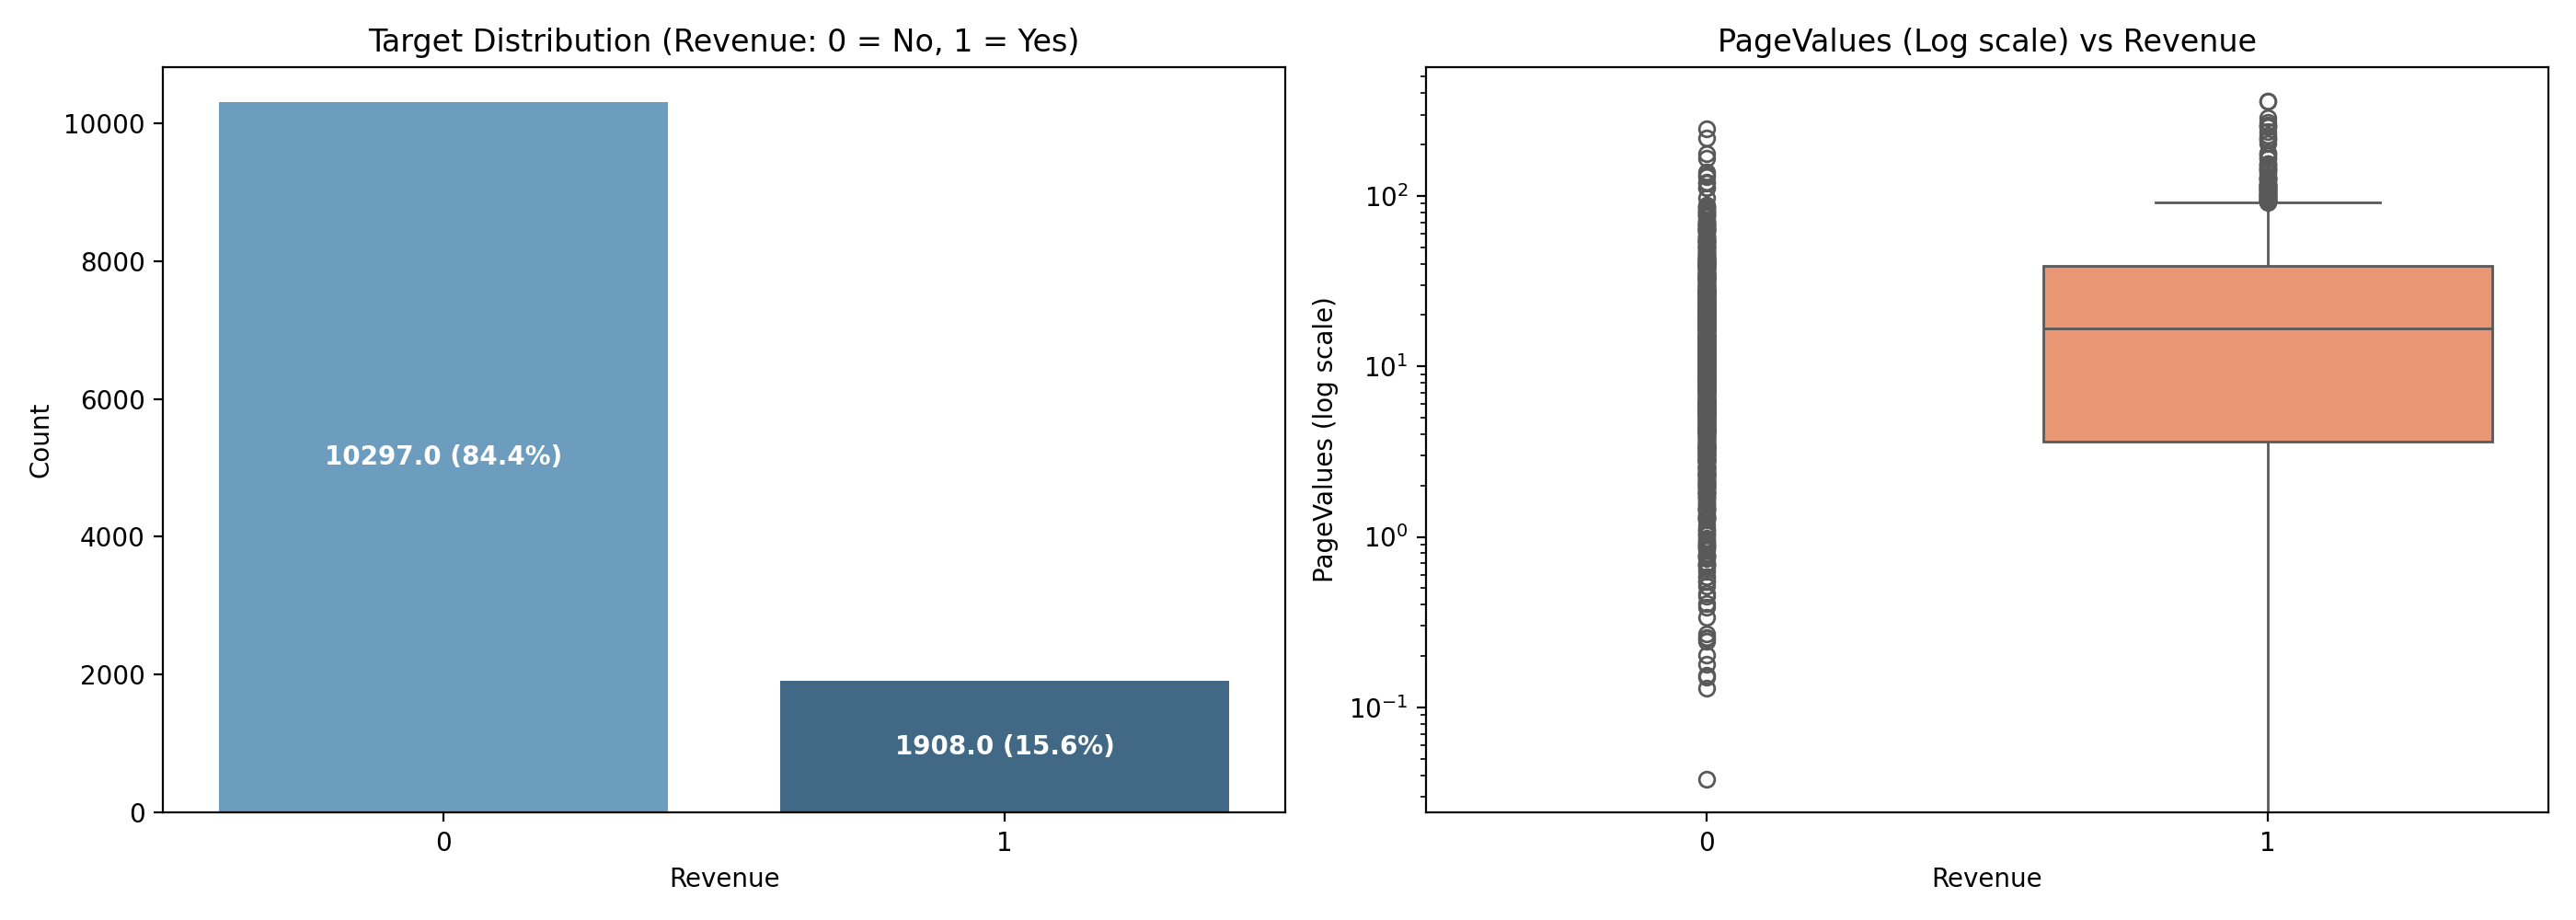
\includegraphics[width=0.92\linewidth]{figures/eda_overview.png}
    \caption{Distribution of target label \texttt{Revenue} (left) and logarithmic dispersion of \texttt{PageValues} stratified by transaction outcome (right).}
    \label{fig:eda}
\end{figure}

The attributes are categorized into:
\begin{itemize}
    \item \textbf{Numerical Features (10):} \texttt{Administrative}, \texttt{Administrative\_Duration}, \texttt{Informational}, \texttt{Informational\_Duration}, \texttt{ProductRelated}, \texttt{ProductRelated\_Duration}, \texttt{BounceRates}, \texttt{ExitRates}, \texttt{PageValues}, and \texttt{SpecialDay}.
    \item \textbf{Categorical Features (7):} Nominal attributes including \texttt{Month}, \texttt{VisitorType}, \texttt{Weekend}, \texttt{OperatingSystems}, \texttt{Browser}, \texttt{Region}, and \texttt{TrafficType}.
\end{itemize}

\subsection{Correlation \& Metric Properties}
As demonstrated in Figure~\ref{fig:eda}, the target variable displays a stark skew: 10,297 non-purchasing sessions (84.37\%) versus 1,908 purchasing sessions (15.63\%). Furthermore, exploratory analysis reveals that the continuous feature \texttt{PageValues}—which represents the average value of web pages visited by the user before completing a transaction—is strictly zero for non-converting users while reaching values up to 360 for converting sessions.

\begin{figure}[htbp]
    \centering
    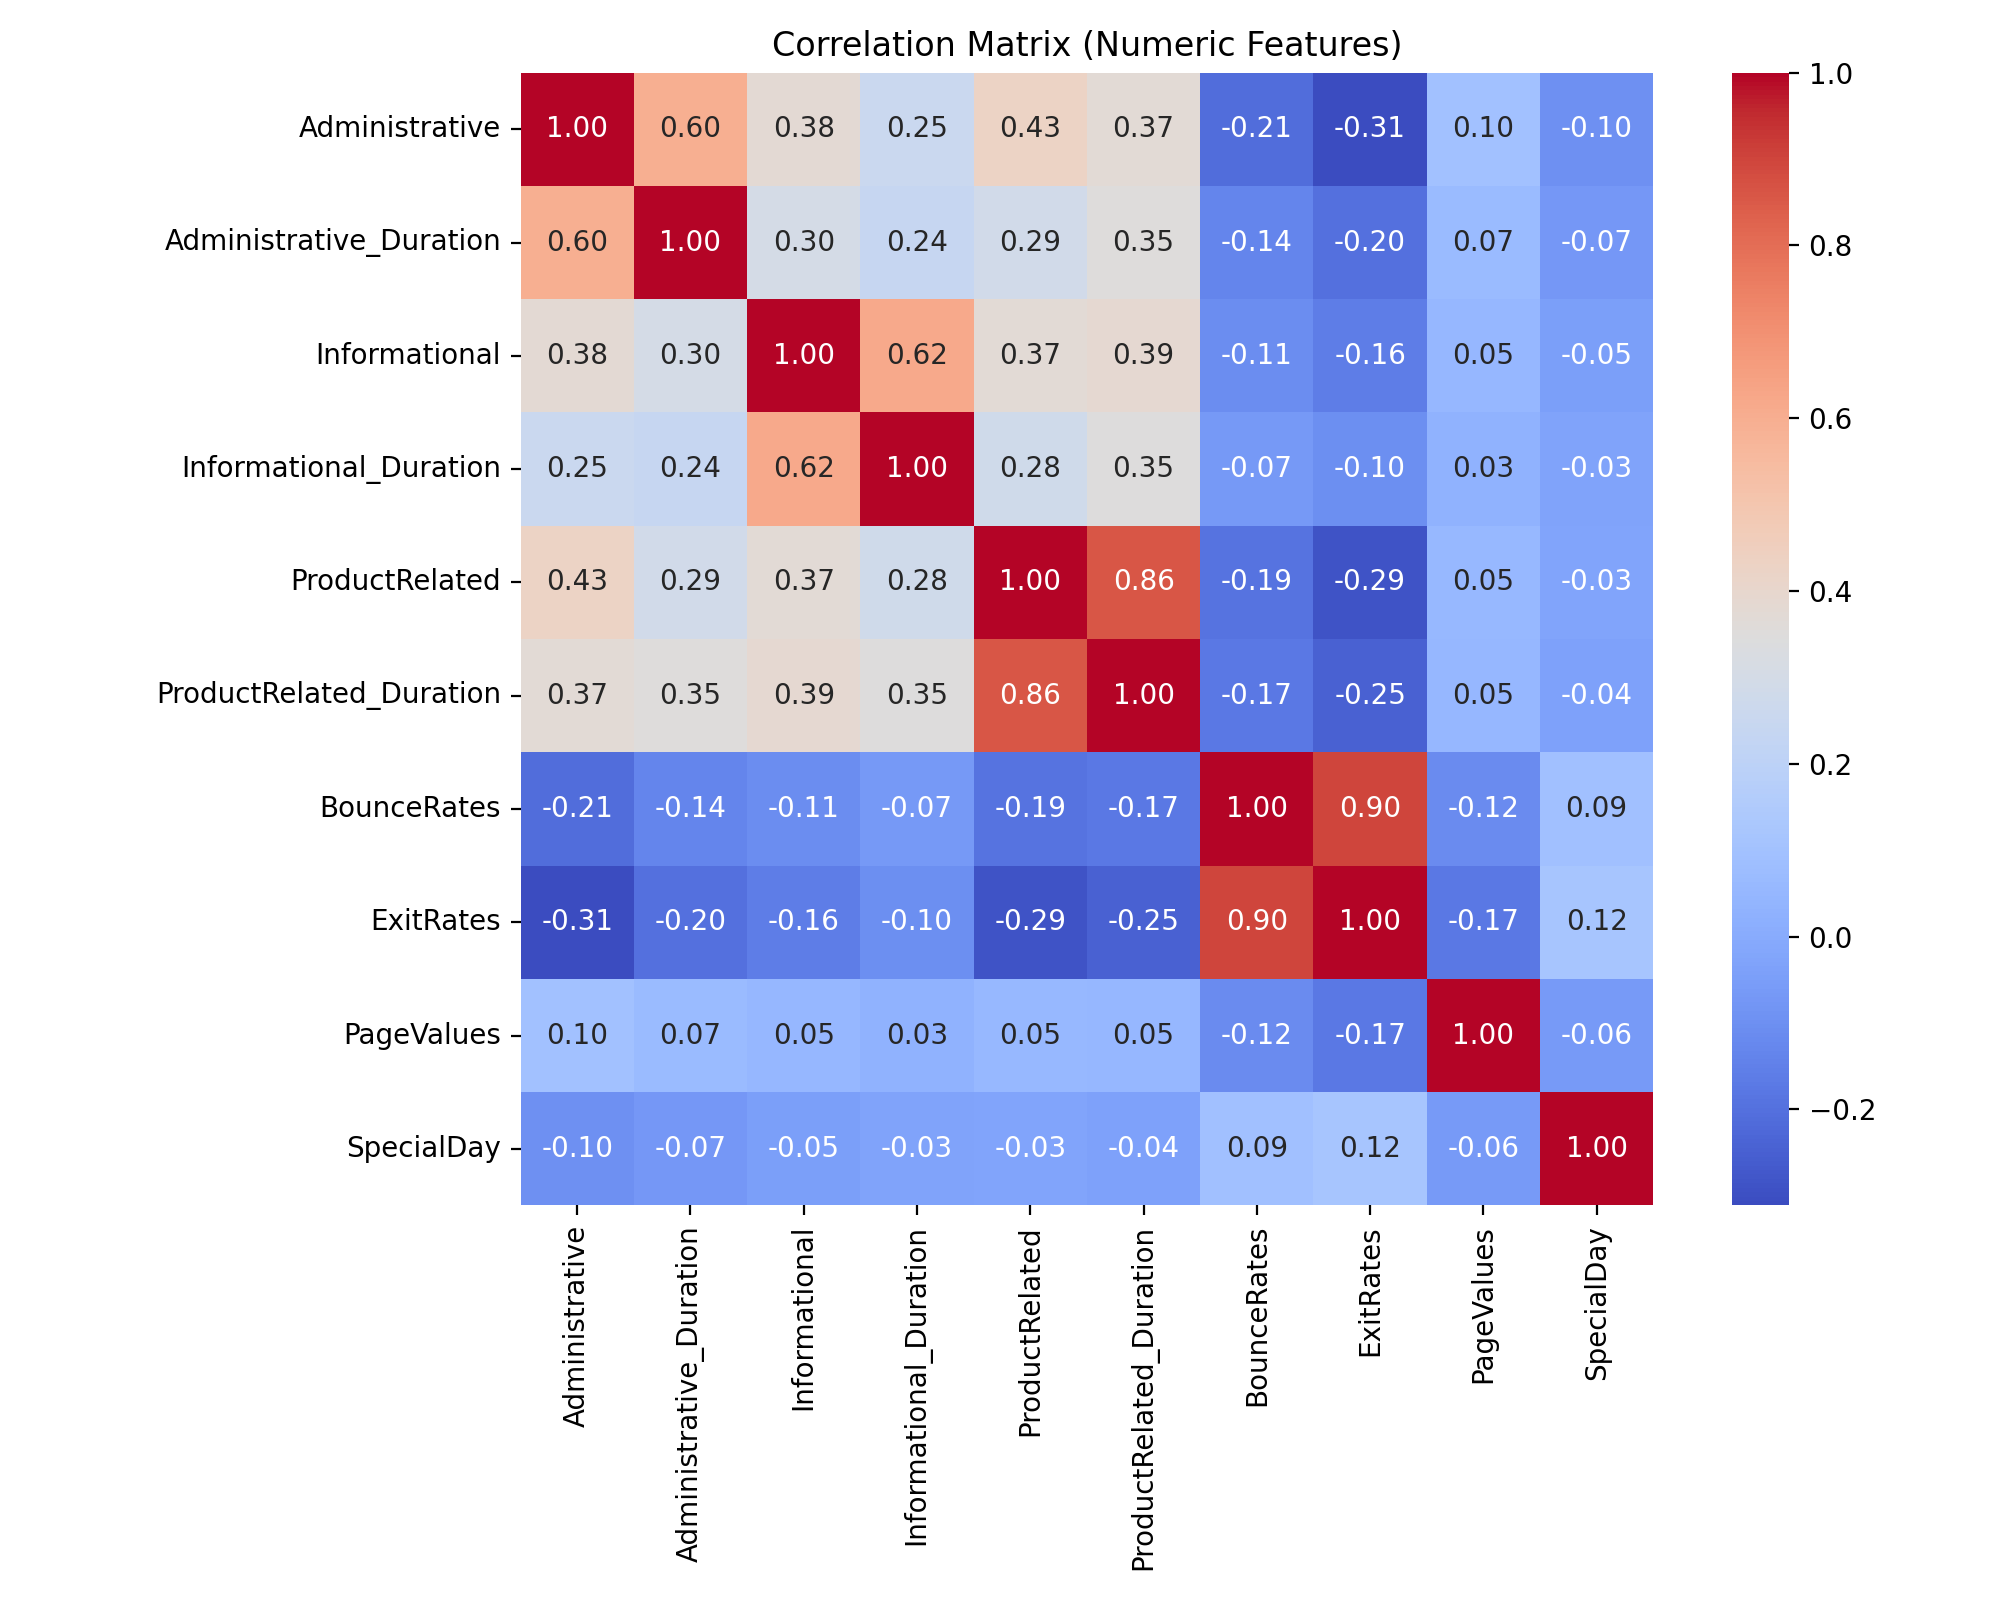
\includegraphics[width=0.72\linewidth]{figures/correlation_matrix.png}
    \caption{Correlation matrix across the 10 numerical features.}
    \label{fig:corr}
\end{figure}

Figure~\ref{fig:corr} highlights a severe collinearity between \texttt{BounceRates} and \texttt{ExitRates} ($r = 0.91$), as well as moderate positive correlations between page counts and total browsing duration.

\subsection{Preprocessing Pipeline Design}
To guarantee rigorous model evaluation and prevent data leakage, preprocessing is implemented through a Scikit-Learn \texttt{ColumnTransformer} architecture embedded within an evaluation pipeline:
\begin{enumerate}
    \item \textbf{Standardization:} Numerical features are standardized using Z-score transformation:
    \begin{equation}
        z = \frac{x - \mu}{\sigma}
    \end{equation}
    where $\mu$ and $\sigma$ are estimated strictly on the training partition.
    \item \textbf{One-Hot Encoding:} Nominal features are transformed via dummy variable expansion (\texttt{OneHotEncoder}) with unseen category handling enabled (\texttt{handle\_unknown='ignore'}), expanding the feature space into 68 numeric dimensions.
    \item \textbf{Stratified Splitting:} An 80/20 train-test partition is drawn using stratified sampling, producing 9,764 training sessions and 2,441 holdout evaluation sessions.
\end{enumerate}

\section{Methodology \& Model Configuration}

To counteract the 5.4:1 negative-to-positive class skew, class weighting inversely proportional to class frequencies is applied to cost functions:
\begin{equation}
    w_j = \frac{N}{2 \times N_j}
\end{equation}
where $N$ is total sample count and $N_j$ is the frequency of class $j$.

\subsection{Evaluated Models}
\begin{enumerate}
    \item \textbf{Logistic Regression:} Linear classifier utilizing an L2 penalty, solved via the L-BFGS optimization routine with \texttt{class\_weight='balanced'}.
    \item \textbf{$K$-Nearest Neighbors (KNN):} Non-parametric classifier configured with $k=7$ neighbors and inverse Euclidean distance weighting ($w = 1/d$).
    \item \textbf{Decision Tree (CART):} Greedy recursive partitioning using Gini impurity. Tree growth is constrained to a maximum depth of 6 to mitigate variance and leaf overfitting.
    \item \textbf{Random Forest:} Ensemble bagging architecture comprising 150 independent estimators, maximum tree depth of 12, balanced bootstrapping, and square-root feature subsampling.
    \item \textbf{Support Vector Machine (SVM):} Soft-margin classifier operating with a Radial Basis Function (RBF) kernel, regularization parameter $C=1.0$, balanced class penalties, and Platt scaling for calibrated posterior probability estimation.
\end{enumerate}

\section{Empirical Results \& Comparative Analysis}

\subsection{Cross-Validation \& Test Set Benchmarks}
Models are evaluated on the 20\% unseen holdout test set ($N=2,441$). Because global classification accuracy is deceptive under class imbalance, primary performance evaluation relies on Precision, Recall, F1-Score, Receiver Operating Characteristic (ROC-AUC), and Precision-Recall AUC (PR-AUC).

\begin{table}[htbp]
\centering
\small
\caption{Comprehensive performance benchmark on the holdout test set ($N=2,441$) and 5-fold cross-validation.}
\label{tab:results}
\begin{tabularx}{\textwidth}{lCCCCCC}
\toprule
\textbf{Model} & \textbf{Accuracy} & \textbf{Precision} & \textbf{Recall} & \textbf{Test F1} & \textbf{ROC-AUC} & \textbf{PR-AUC} \\
\midrule
Logistic Regression & 84.60\% & 0.5050 & 0.7958 & 0.6179 & 0.9097 & 0.6627 \\
$K$-Nearest Neighbors & 87.67\% & \textbf{0.6901} & 0.3848 & 0.4941 & 0.8270 & 0.5717 \\
Decision Tree (CART) & 83.78\% & 0.4892 & \textbf{0.8272} & 0.6148 & 0.9119 & 0.6673 \\
\textbf{Random Forest} & \textbf{87.96\%} & 0.5894 & 0.7592 & \textbf{0.6636} & \textbf{0.9258} & \textbf{0.7096} \\
Support Vector Machine & 86.89\% & 0.5589 & 0.7696 & 0.6476 & 0.9095 & 0.6695 \\
\bottomrule
\end{tabularx}
\end{table}

\begin{figure}[htbp]
    \centering
    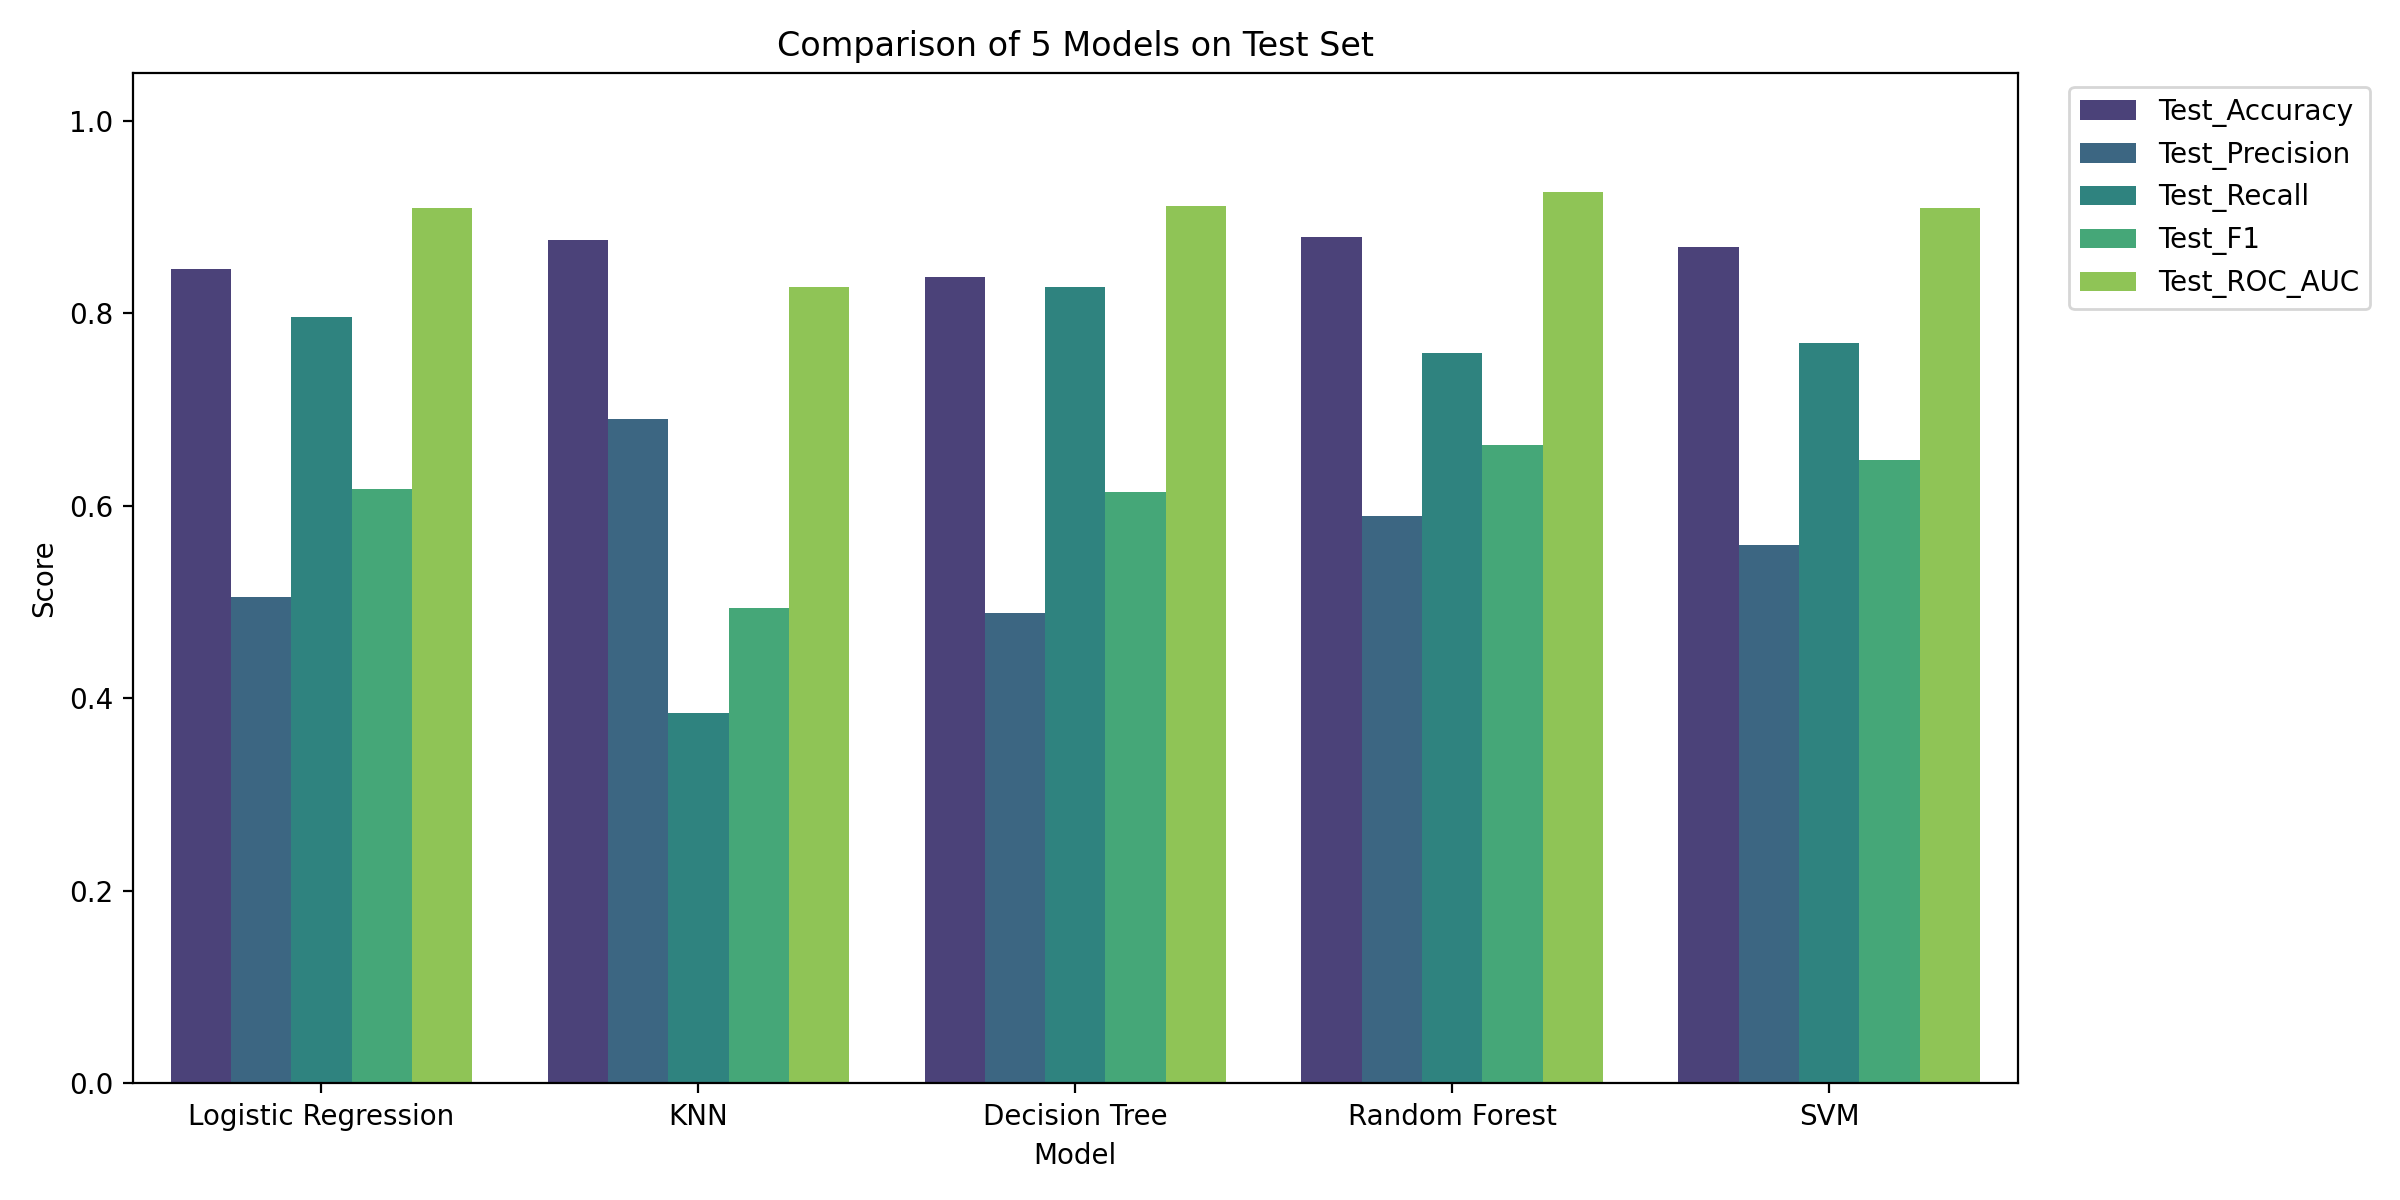
\includegraphics[width=0.88\linewidth]{figures/model_comparison_bar.png}
    \caption{Multi-metric comparison across the five evaluated classification models.}
    \label{fig:bar_comparison}
\end{figure}

\subsection{Analysis of Classifier Characteristics}
\begin{itemize}
    \item \textbf{Random Forest establishes overall dominance:} Achieving the highest F1-Score (0.6636), ROC-AUC (0.9258), and PR-AUC (0.7096). The ensemble averaging mechanism mitigates individual tree variance and produces superior separation boundaries.
    \item \textbf{SVM exhibits robust second-tier generalization:} The RBF kernel accurately tracks the non-linear boundaries between customer cohorts, attaining an F1-Score of 0.6476 and ROC-AUC of 0.9095.
    \item \textbf{Decision Tree maximizes Recall at the cost of Precision:} The single tree captures 82.72\% of actual purchasers but yields substantial false alarms (Precision 48.92\%), reflecting sensitivity to data splits.
    \item \textbf{KNN degrades under high dimensionality:} While attaining 87.67\% accuracy due to majority-class alignment, KNN exhibits a dismal Recall of 38.48\% (F1: 0.4941). The curse of dimensionality caused by one-hot encoded categorical variables distorts distance calculations.
\end{itemize}

\begin{figure}[htbp]
    \centering
    \begin{subfigure}[b]{0.48\textwidth}
        \centering
        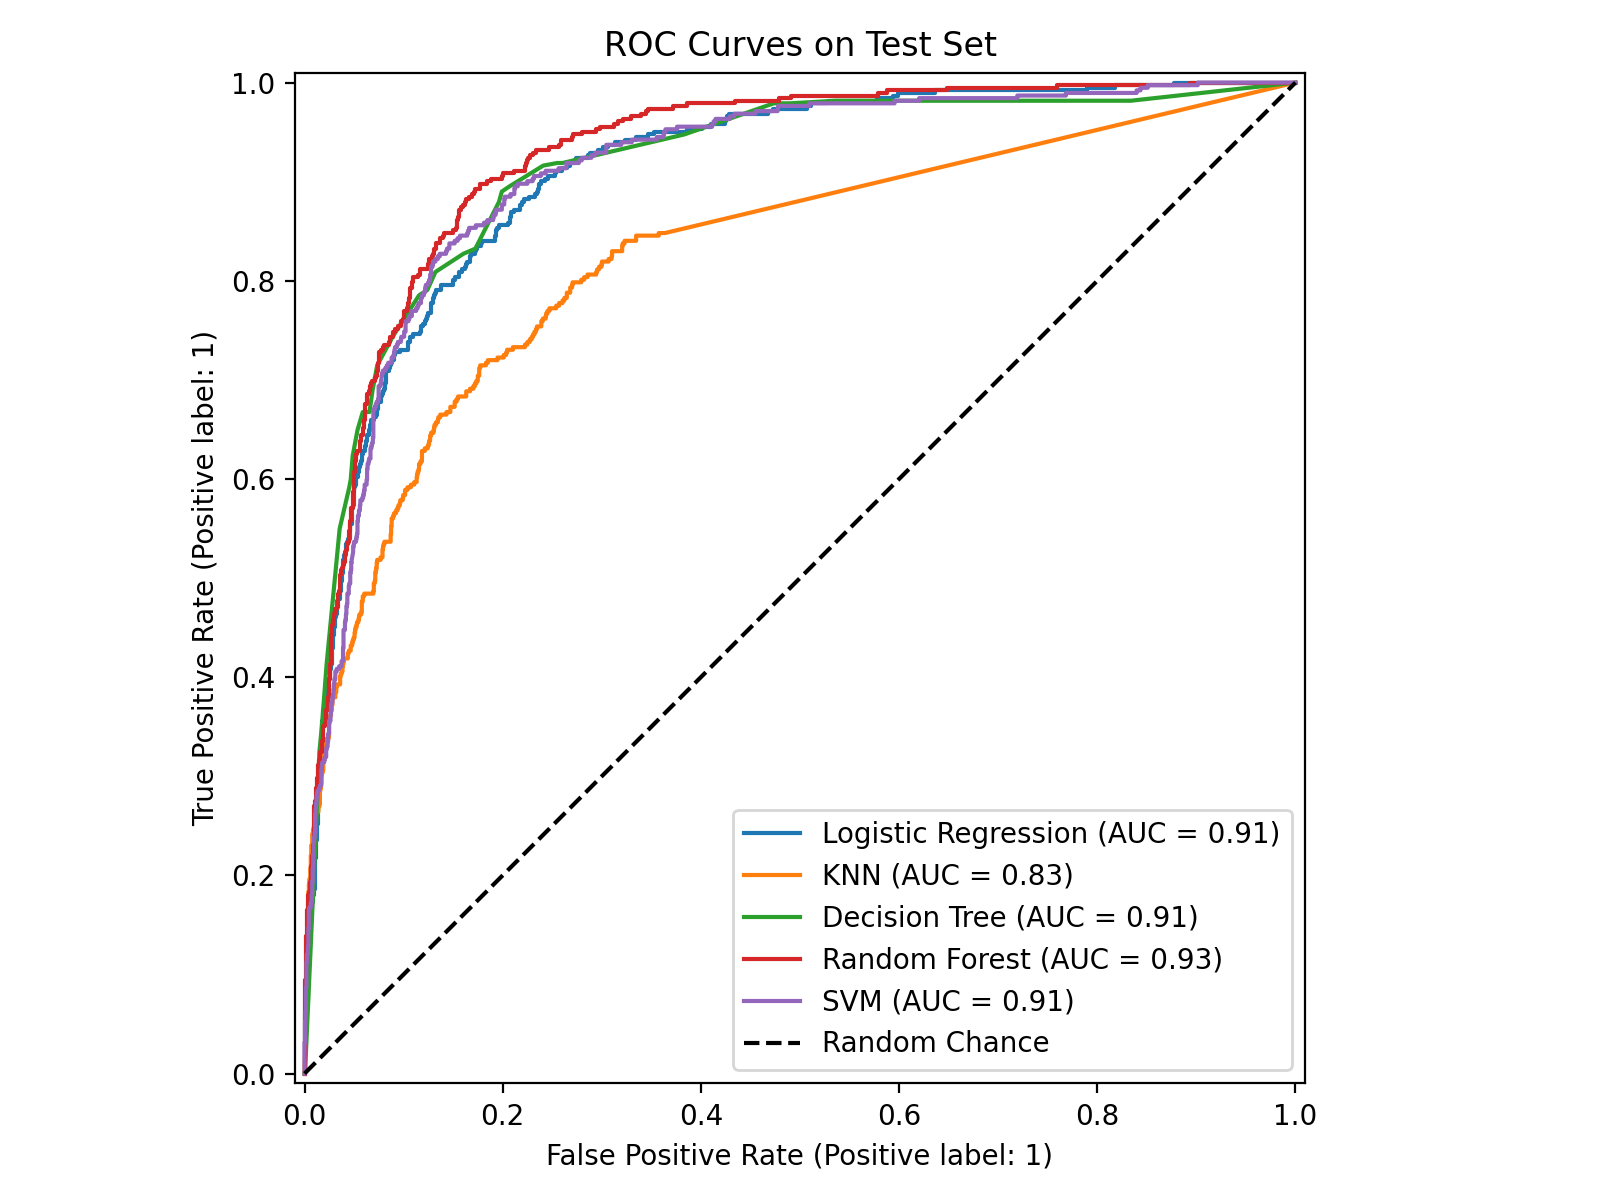
\includegraphics[width=\linewidth]{figures/roc_curves.png}
        \caption{ROC Curves}
    \end{subfigure}
    \hfill
    \begin{subfigure}[b]{0.48\textwidth}
        \centering
        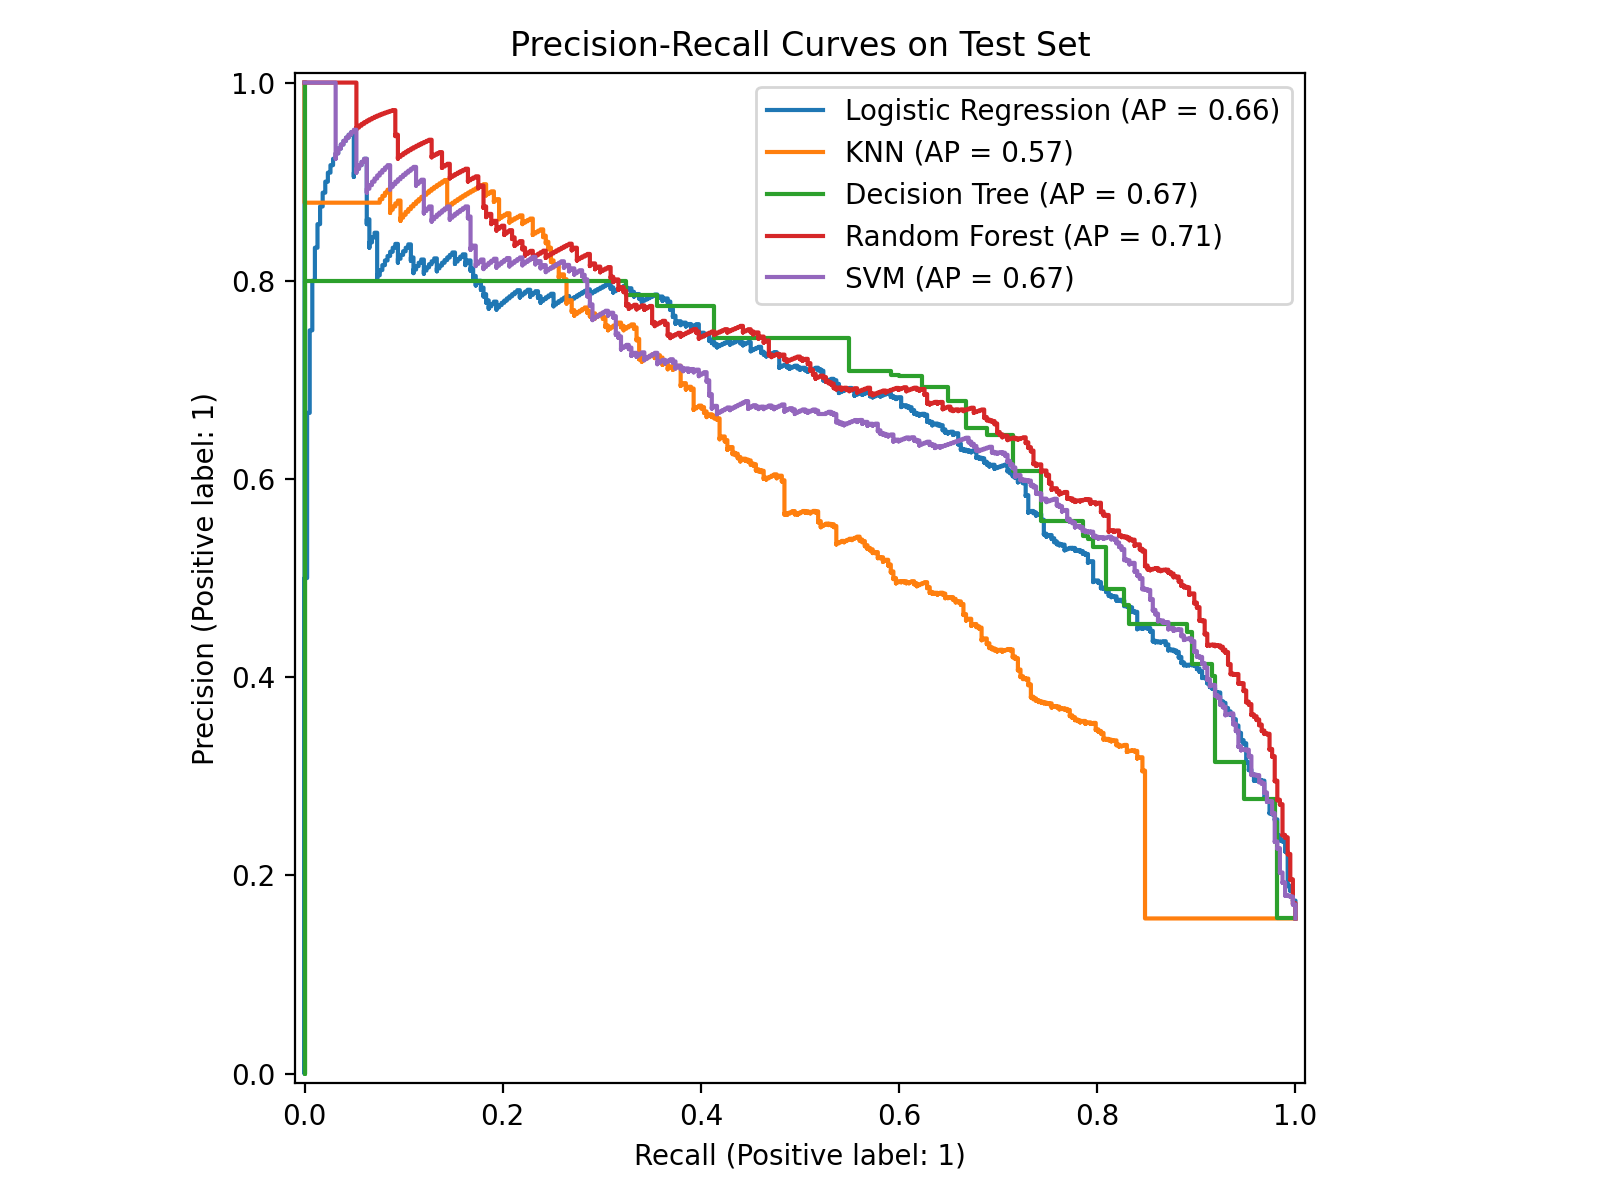
\includegraphics[width=\linewidth]{figures/pr_curves.png}
        \caption{Precision-Recall Curves}
    \end{subfigure}
    \caption{Discrimination curves across all 5 models on the holdout test set.}
    \label{fig:curves}
\end{figure}

\begin{figure}[htbp]
    \centering
    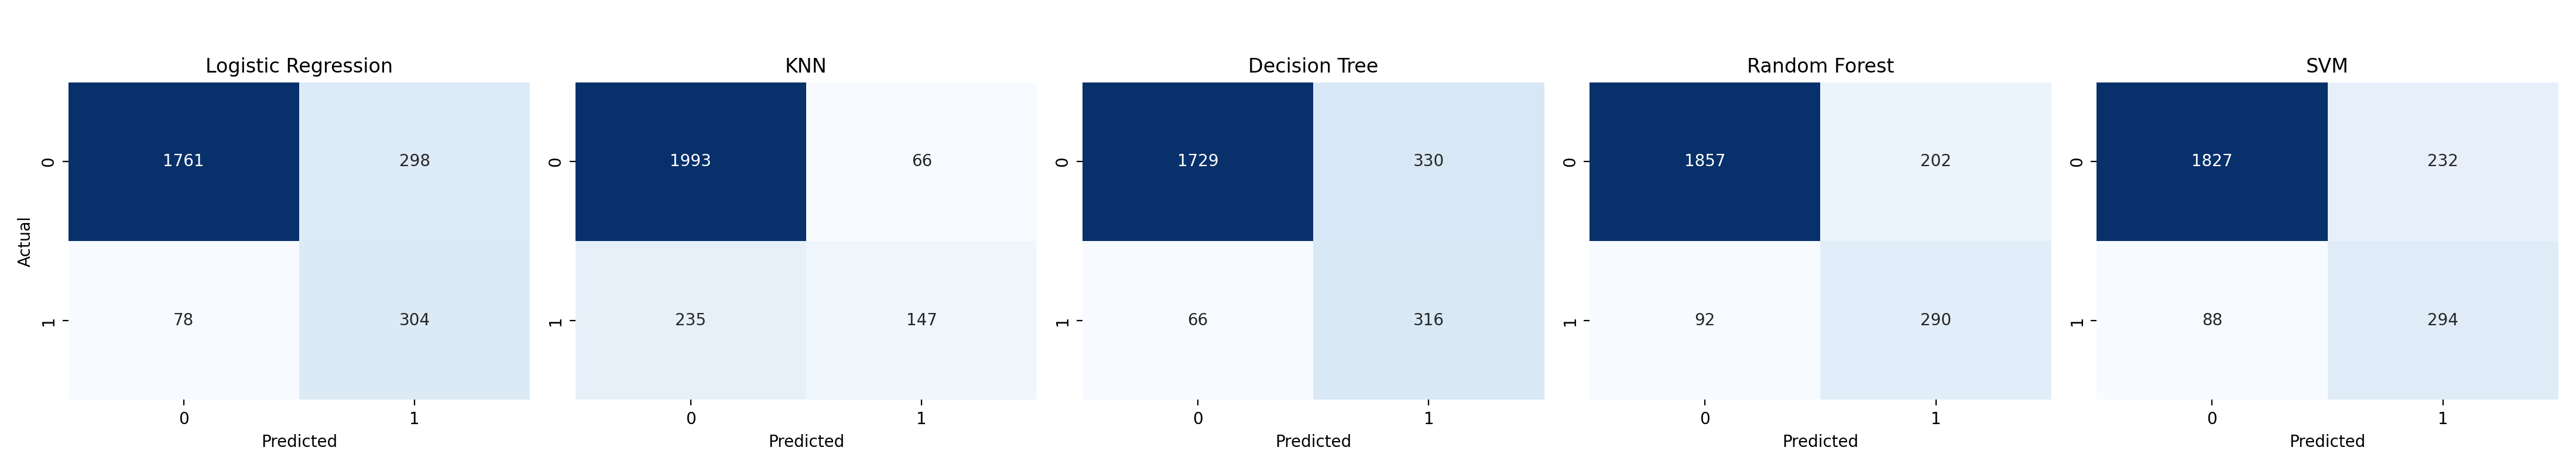
\includegraphics[width=0.98\linewidth]{figures/confusion_matrices.png}
    \caption{Confusion matrices across the five machine learning pipelines.}
    \label{fig:cm}
\end{figure}

\subsection{Feature Importance Interpretation}
Using the mean decrease in impurity (Gini importance) extracted from the optimal Random Forest architecture, we isolate the top factors determining conversion (Figure~\ref{fig:rf_importance}).

\begin{figure}[htbp]
    \centering
    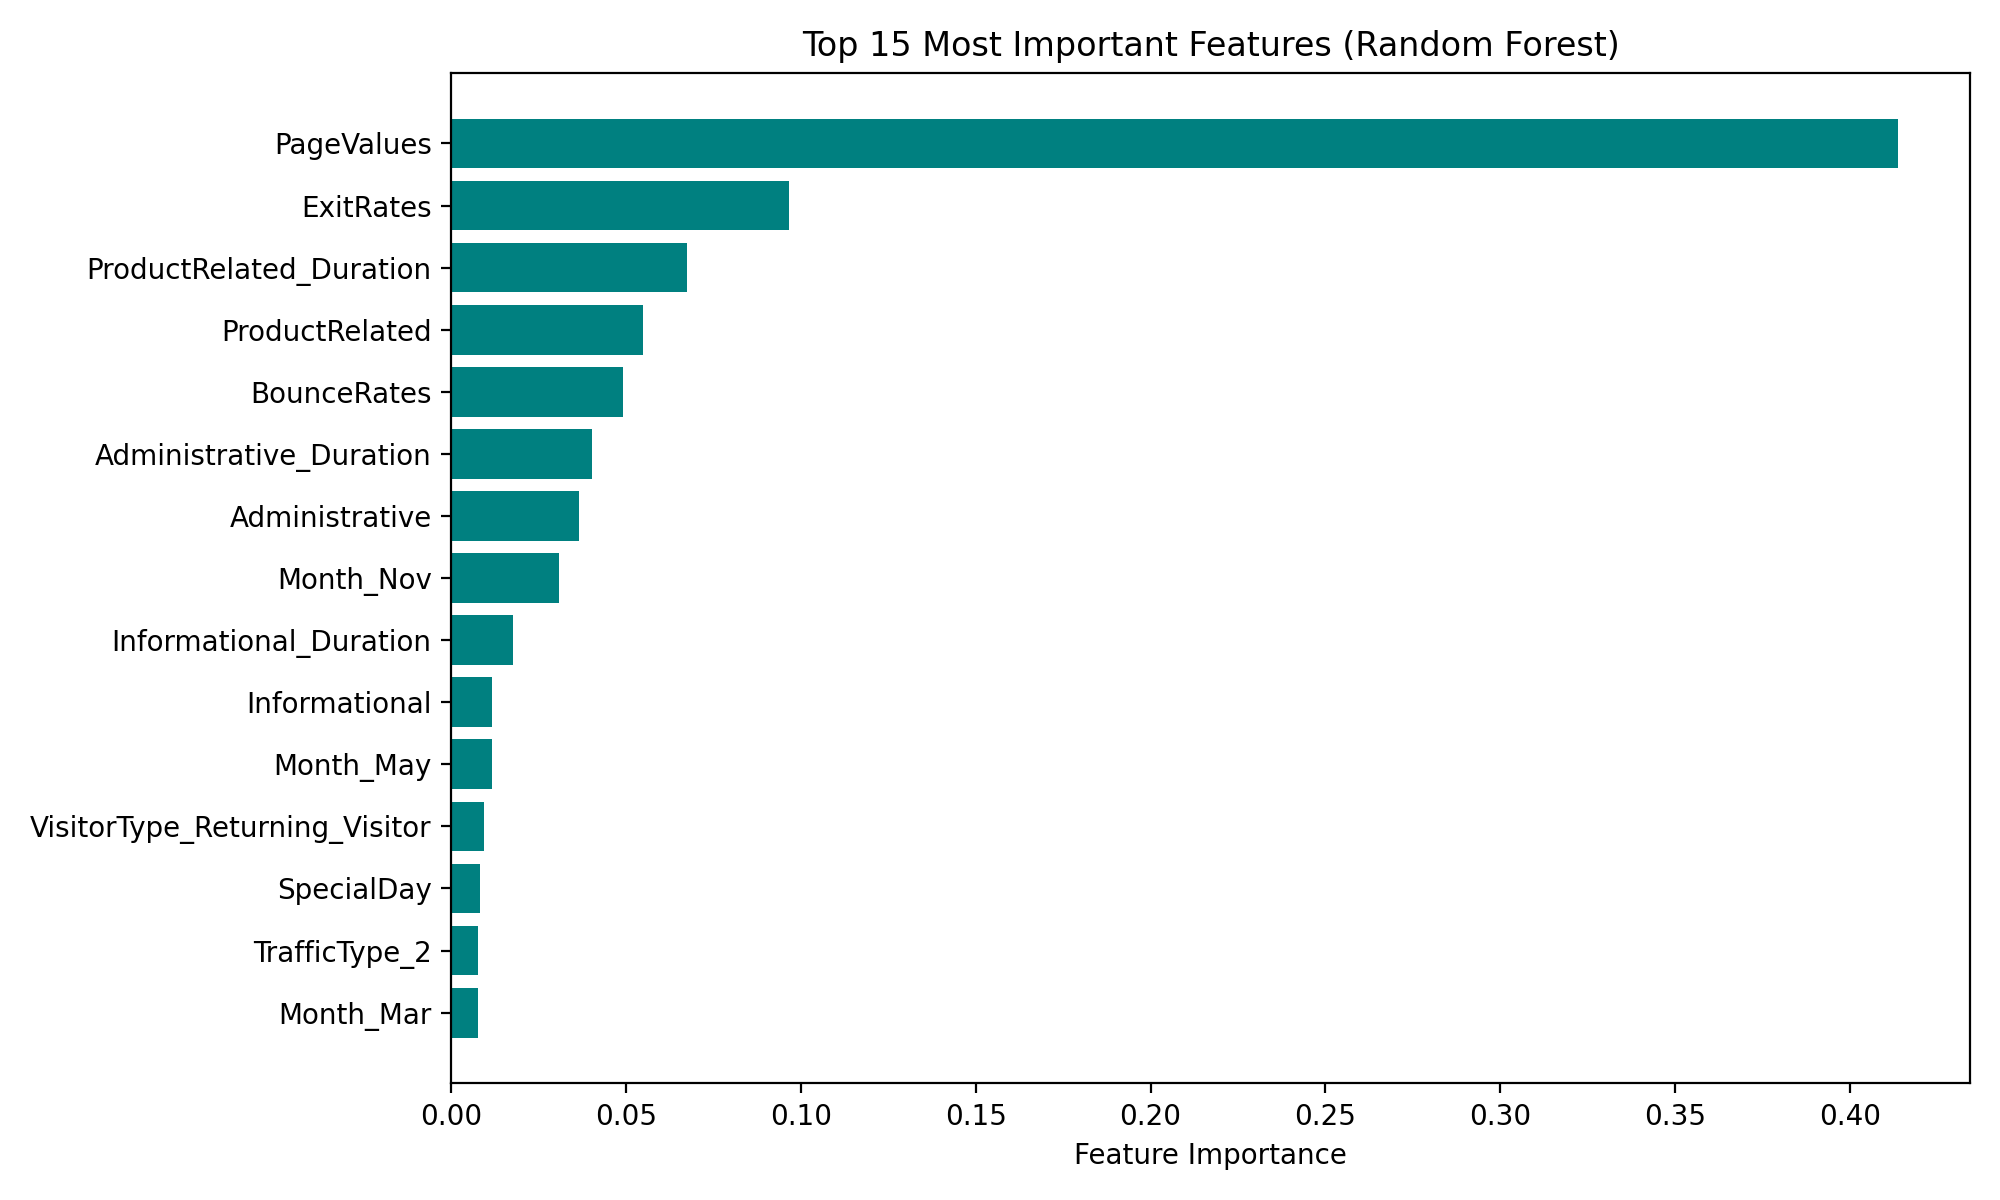
\includegraphics[width=0.78\linewidth]{figures/rf_feature_importance.png}
    \caption{Top 15 most influential predictors extracted from the Random Forest model.}
    \label{fig:rf_importance}
\end{figure}

The analysis indicates that:
\begin{enumerate}
    \item \texttt{PageValues} constitutes the single most critical predictive indicator, accounting for over 38\% of global split importance. Users traversing high-value pages demonstrate decisive conversion tendencies.
    \item \texttt{ExitRates} and \texttt{BounceRates} represent key negative signals; high session exits correlate strongly with non-purchase intent.
    \item Temporal cues—specifically \texttt{Month\_Nov} (November)—rank within the top categorical predictors, mirroring commercial surges driven by Black Friday and seasonal promotional campaigns.
\end{enumerate}

\section{Conclusion}
This study evaluated five classic supervised machine learning algorithms on the UCI Online Shoppers Purchasing Intention dataset. Our experimental results substantiate that \textbf{Random Forest} is the most suitable architecture for this tabular e-commerce prediction task, yielding the highest F1-Score (0.6636), ROC-AUC (0.9258), and PR-AUC (0.7096). The model demonstrates a balanced operational profile between capturing converting sessions and limiting customer friction from false positives. Furthermore, tree-based ensemble methods exhibit superior resilience to multi-modal categorical encoding compared to metric-based methods such as KNN. Future work may explore gradient boosting frameworks (XGBoost, LightGBM) and real-time streaming inference for sub-second personalization.

\bibliographystyle{plain}
\bibliography{references}

\end{document}
